\chapter{Pianificazione}\label{Pianificazione}
Il gruppo \textit{Jawa Druids} ha pianificato le attività di progetto seguendo le scadenze riportate nel capitolo \ref{IntroduzioneScadenze}. Il progetto è dunque suddiviso nelle seguenti fasi:
\begin{itemize}
	\item Analisi;
	\item Consolidamento dei requisiti$_{\scaleto{G}{3pt}}$;
	\item Progettazione architetturale;
	\item Progettazione di dettaglio e codifica;
	\item Validazione e collaudo.
\end{itemize}
Ognuna di queste fasi è formata da attività$_{\scaleto{G}{3pt}}$ illustrate nei diagrammi di Gantt$_G$, che permettono la rappresentazione grafica di un calendario, utile al fine di pianificare, coordinare e tracciare specifiche attività dando una chiara illustrazione del suo stato di avanzamento.
\section{Analisi}\label{PianificazioneAnalisi}
\textbf{Periodo:} dal 22-11-2020 al 11-01-2021.\\
Questo periodo ha inizio con la formazione dei gruppi e termina con la scadenza per la consegna dei documenti relativi alla Revisione dei Requisiti.
Le principali attività$_{\scaleto{G}{3pt}}$ svolte in questo periodo riguardano l'analisi dei requisiti$_{\scaleto{G}{3pt}}$ posti dal proponente, la pianificazione, la scelta di metriche adeguate per il \textit{Piano di Qualifica} e la stesura della documentazione necessaria a supporto del progetto stesso, come riportato in seguito:
\begin{itemize}
	\item \textbf{Studio di Fattibilità:} attività$_{\scaleto{G}{3pt}}$ di studio di tutti i capitolati$_{\scaleto{G}{3pt}}$, elencando per ciascuno i punti positivi e negativi che li caratterizzano. Si specificano inoltre le motivazioni riguardanti la scelta del capitolato$_{\scaleto{G}{3pt}}$ \textit{GDP: Gathering Detection Platform}.
	Questa attività$_{\scaleto{G}{3pt}}$ è bloccante per l'inizio dell'\textit{Analisi dei Requisiti};
	\item \textbf{Norme di Progetto:} definisce tutte le regole, convenzioni e tecnologie che il gruppo \textit{Jawa Druids} deve rispettare ed utilizzare durante lo sviluppo dell'intero progetto;
	\item \textbf{Glossario:} racchiude termini che possono risultare ambigui durante lo svolgimento del progetto, con annessa una breve descrizione;
	\item \textbf{Piano di Progetto:} il presente documento in cui le attività$_{\scaleto{G}{3pt}}$, i compiti$_{\scaleto{G}{3pt}}$, e le risorse precedentemente analizzate vengono distribuite tra i componenti di \textit{Jawa Druids}. Presenta inoltre il calcolo del preventivo e le scadenze che il gruppo intende rispettare;
	\item \textbf{Lettera di Presentazione:} lettera in cui il gruppo \textit{Jawa Druids} si candida ufficialmente come fornitore$_{\scaleto{G}{3pt}}$ del prodotto software richiesto;
	\item \textbf{Analisi dei requisiti:} studio ed analisi dei requisiti$_{\scaleto{G}{3pt}}$ del capitolato$_{\scaleto{G}{3pt}}$ scelto nello \textit{Studio di Fattibilità};
	\item \textbf{Piano di qualifica:} documento in cui vengono indicate le strategie di verifica e validazione che il gruppo adotta per garantire la qualità del prodotto software.
\end{itemize}
\subsection{Diagramma di Gantt: Analisi}\label{PianificazioneDiagrammaDiGanttAnalisi}
\begin{figure}[!h]
	\begin{center}
		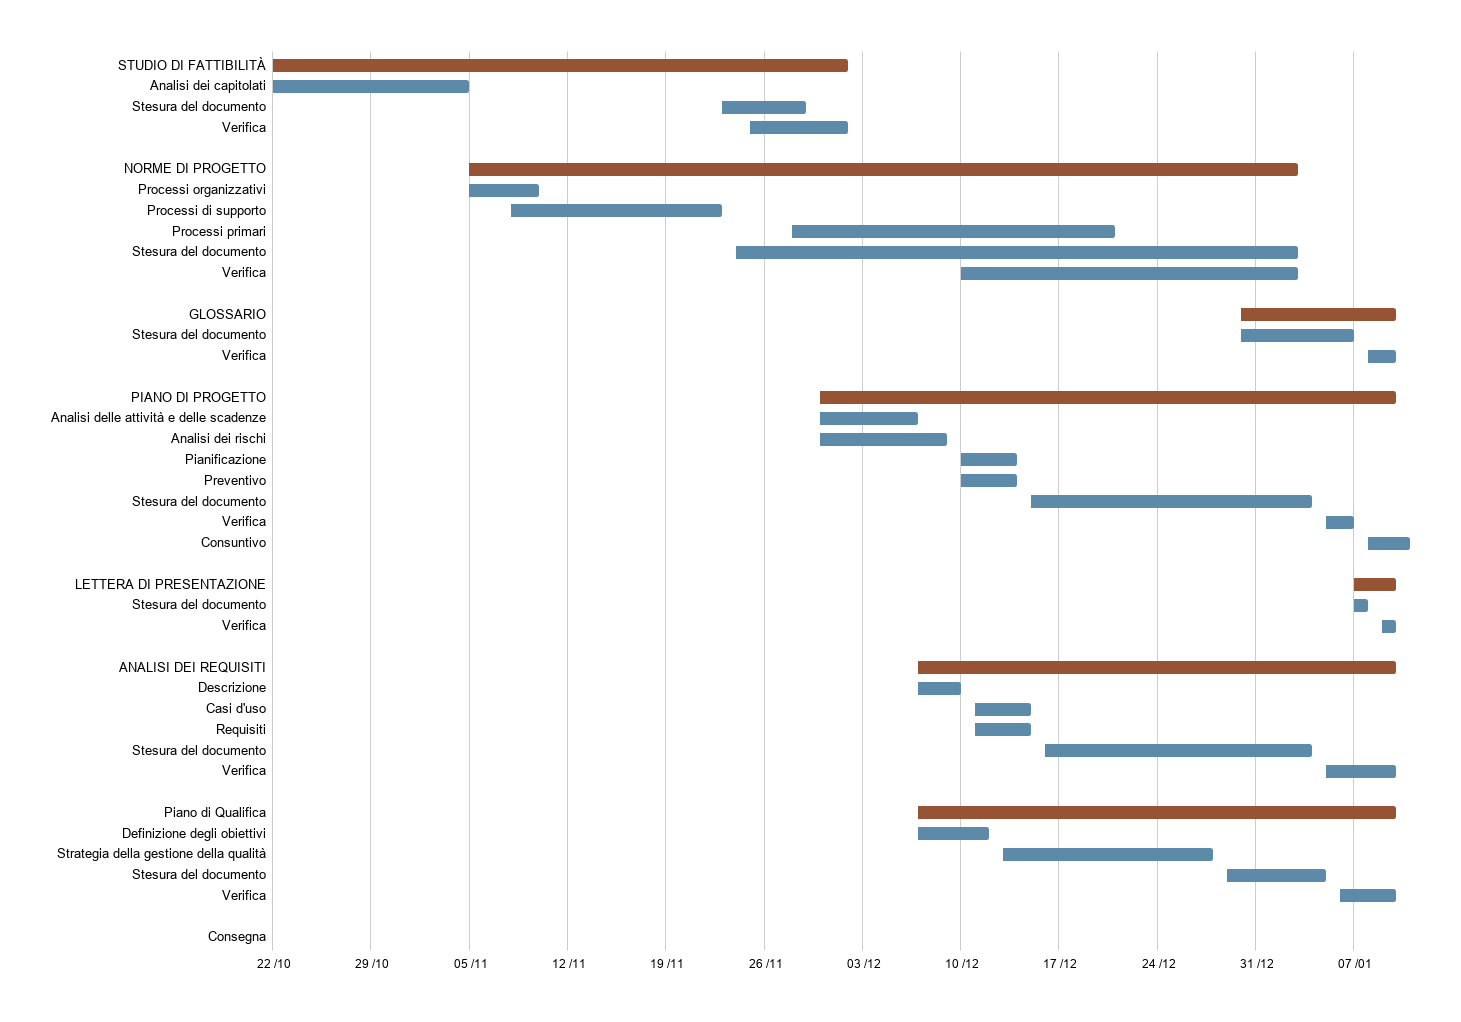
\includegraphics[width=1\linewidth]{../immagini/pdp/gantt_analisi.png}
		\caption{Diagramma di Gantt dell'attività di analisi}
	\end{center}
\end{figure}

\section{Consolidamento dei requisiti}\label{PianificazioneConsolidamentoDeiRequisiti}
\textbf{Periodo:} dal 11-01-2021 al 18-01-2021
Questo periodo ha inizio subito dopo il termine del precedente e finisce con la presentazione della Revisione dei Requisiti.
Il gruppo \textit{Jawa Druids} si dedicherà ai seguenti compiti$_{\scaleto{G}{3pt}}$:
\begin{itemize}
	\item avanzamento con lo studio individuale relativo a:
	\begin{itemize}
		\item acquisizione dei dati;
		\item simulazione dei dati;
		\item machine learning$_G$;
		\item web app.
	\end{itemize}
	\item preparazione del materiale necessario alla presentazione.
\end{itemize}
\subsection{Diagramma di Gantt: consolidamento dei requisiti}\label{PianificazioneDiagrammaDiGanttConsolidamento}
\begin{figure}[!h]
	\begin{center}
		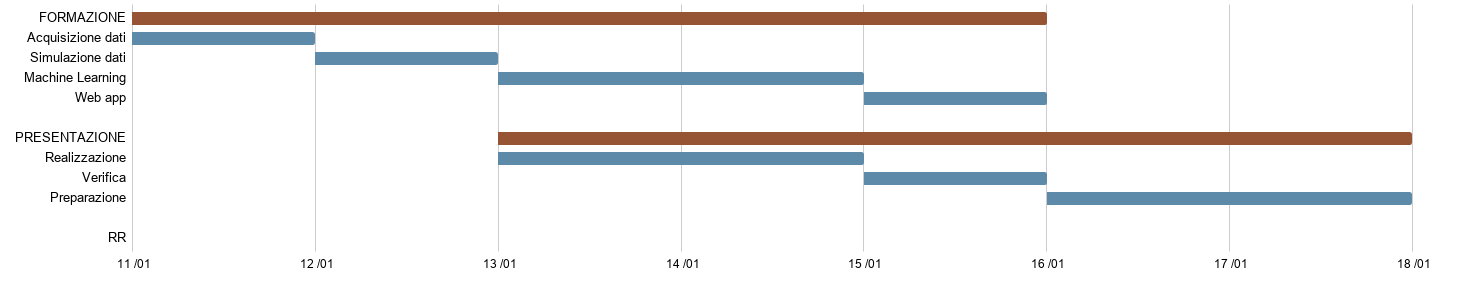
\includegraphics[width=1\linewidth]{../immagini/pdp/gantt_consolidamento_requisiti.png}
		\caption{Diagramma di Gantt del consolidamento dei requisiti}
	\end{center}
\end{figure}
\clearpage
\section{Progettazione architetturale}\label{PianificazioneProgettazioneArchitetturale}
\textbf{Periodo:} dal 18-01-2021 al 08-03-2021. \\
Questo periodo ha inizio subito dopo conclusione del precedente e termina con la Revisione di Progettazione.
Esso porta all'individuazione di una soluzione architetturale che permetta il soddisfacimento dei requisiti$_{\scaleto{G}{3pt}}$ obbligatori. È suddivisa in:
\begin{itemize}
	\item \textbf{Incremento e verifica:} analizzando l'esito della Revisione dei Requisiti, vengono svolte attività$_{\scaleto{G}{3pt}}$ di Incremento e Verifica sui vari documenti redatti, dove necessario;
	\item \textbf{Technology Baseline$_G$:} viene redatta la documentazione di supporto, contenente la descrizione delle tecnologie individuate e il tracciamento della relazione tra le componenti e i requisiti$_{\scaleto{G}{3pt}}$ che vanno a soddisfare.
	Viene realizzato un Proof of Concept$_G$ che verrà condiviso col proponente$_{\scaleto{G}{3pt}}$ per verificare il corretto sviluppo del software.
\end{itemize}
\subsection{Diagramma di Gantt: progettazione architetturale}\label{PianificazioneDiagrammaDiGanttProgettazioneArchitetturale}
\begin{figure}[h]
	\begin{center}
		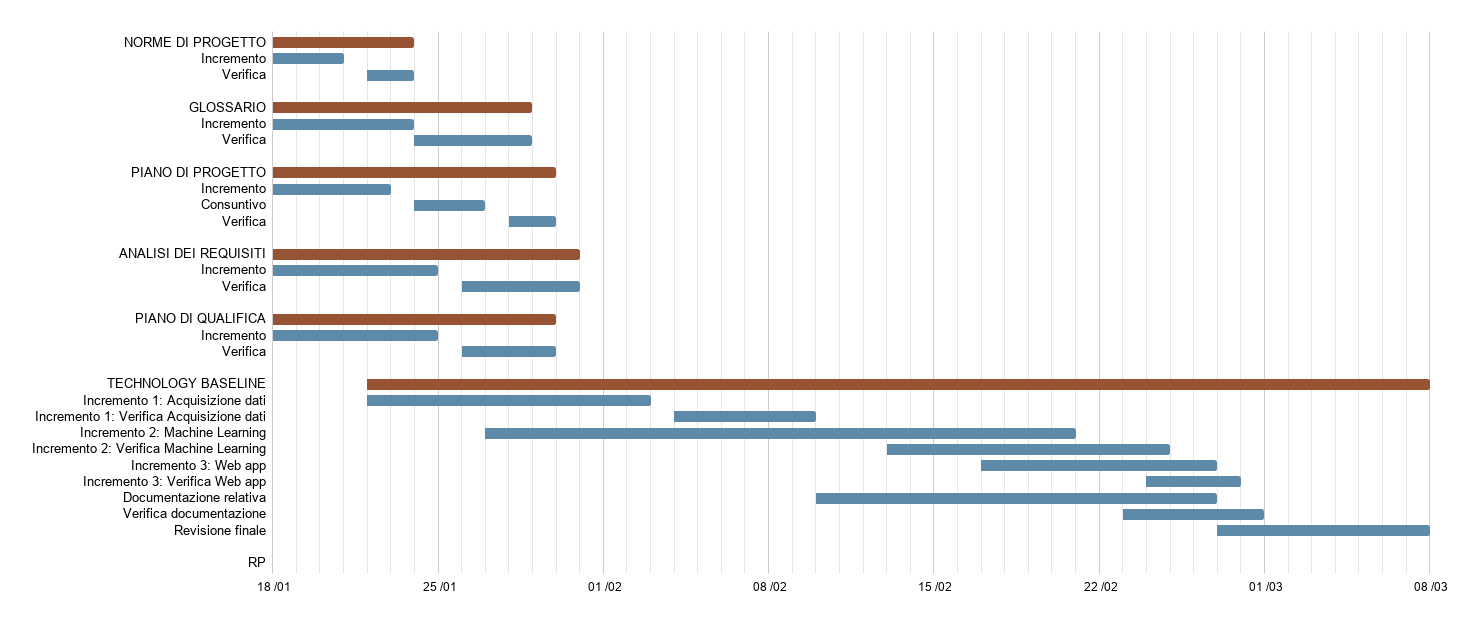
\includegraphics[width=0.9\linewidth]{../immagini/pdp/gantt_progettazione_architetturale.png}
		\caption{Diagramma di Gantt della progettazione architetturale}
	\end{center}
\end{figure}
\clearpage
\section{Progettazione di dettaglio e codifica}\label{PianificazioneProgettazioneDettaglio}
\textbf{Periodo:} dal 15-03-2021 al 09-04-2021
Questo periodo inizia appena concluso il precedente e termina con la Revisione di Qualifica.
Le principali attività$_{\scaleto{G}{3pt}}$ svolte in questo periodo sono
\begin{itemize}
	\item \textbf{Incremento e verifica:} alcuni dei documenti già prodotti vengono migliorati e aggiornati;
	\item \textbf{Product Baseline$_G$:} segue la Technology Baseline$_{\scaleto{G}{3pt}}$, dove vengono studiati meglio design pattern$_G$, classi e attività$_{\scaleto{G}{3pt}}$ necessarie alla codifica;
	\item \textbf{Specifica Tecnica:} è un documento contenente tutte le caratteristiche del prodotto e le motivazioni che hanno portato alla loro scelta;
	\item \textbf{Codifica:} attività$_{\scaleto{G}{3pt}}$ nella quale viene prodotto e verificato il codice;
	\item \textbf{Manuale utente:} attività$_{\scaleto{G}{3pt}}$ nella quale viene redatto il documento contenente le informazioni su come funziona e su come si utilizza il prodotto.
\end{itemize}
\subsection{Diagramma di Gantt: progettazione di dettaglio e codifica}\label{PianificazioneDiagrammaDiGanttProgettazioneDettaglio}
\begin{figure}[!h]
	\begin{center}
		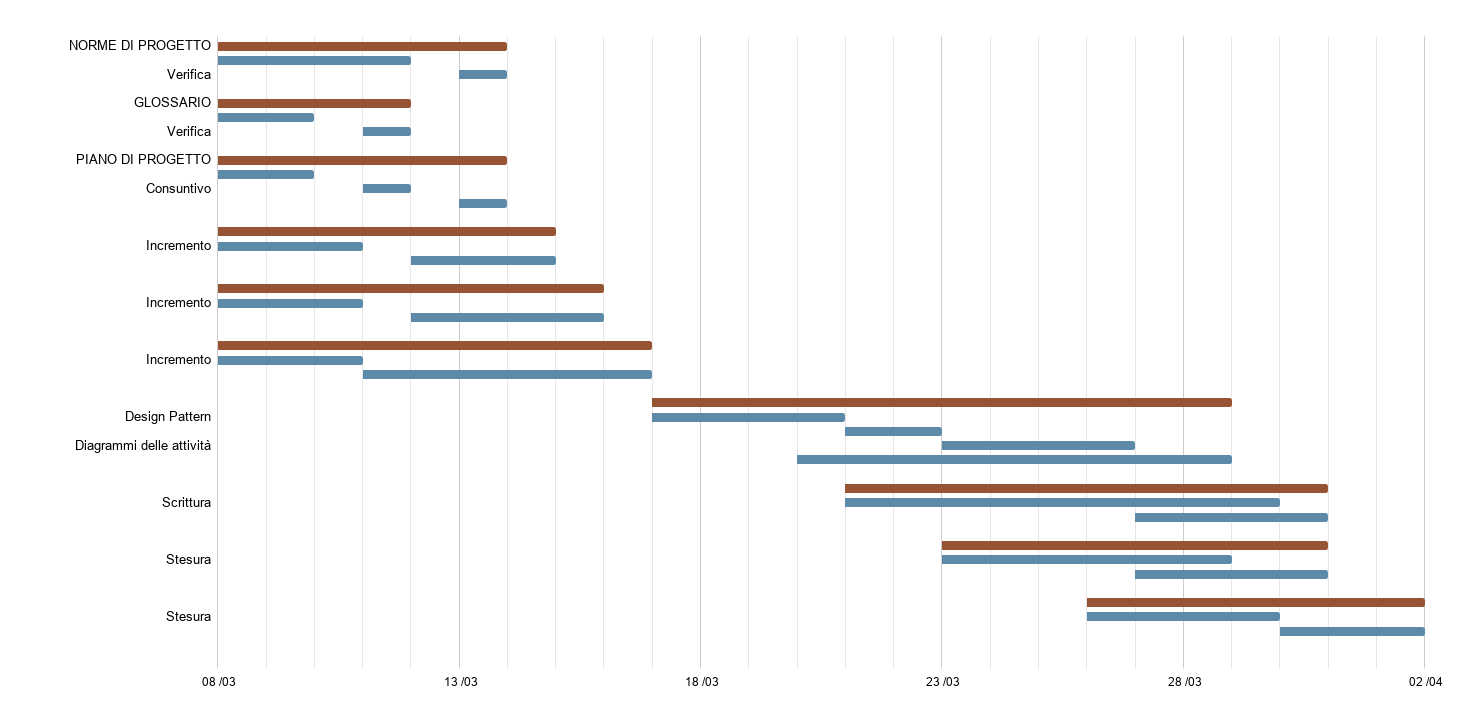
\includegraphics[width=0.8\linewidth]{../immagini/pdp/gantt_progettazione_dettaglio.png}
		\caption{Diagramma di Gantt dell'attività di progettazione di dettaglio e codifica}
	\end{center}
\end{figure}
\section{Validazione e Collaudo}\label{PianificazioneValidazione}
\textbf{Periodo:} dal 16-04-2021 al 10-05-2021
Questo periodo inizia appena concluso il precedente e termina con la Revisione di Accettazione.
Le principali attività$_{\scaleto{G}{3pt}}$ svolte in questo periodo sono:
\begin{itemize}
	\item \textbf{Incremento e verifica:} analizzando l'esito della Revisione di Qualifica vengono svolte attività$_{\scaleto{G}{3pt}}$ di Incremento e Verifica sui vari documenti redatti;
	\item \textbf{Validazione e Collaudo:} vengono realizzati gli ultimi test, con i dovuti controlli finali, in modo da garantire un buon livello di qualità e correttezza.
\end{itemize}
\subsection{Diagramma di Gantt: validazione e collaudo}\label{PianificazioneDiagrammaDiGanttValidazione}
\begin{figure}[!h]
	\begin{center}
		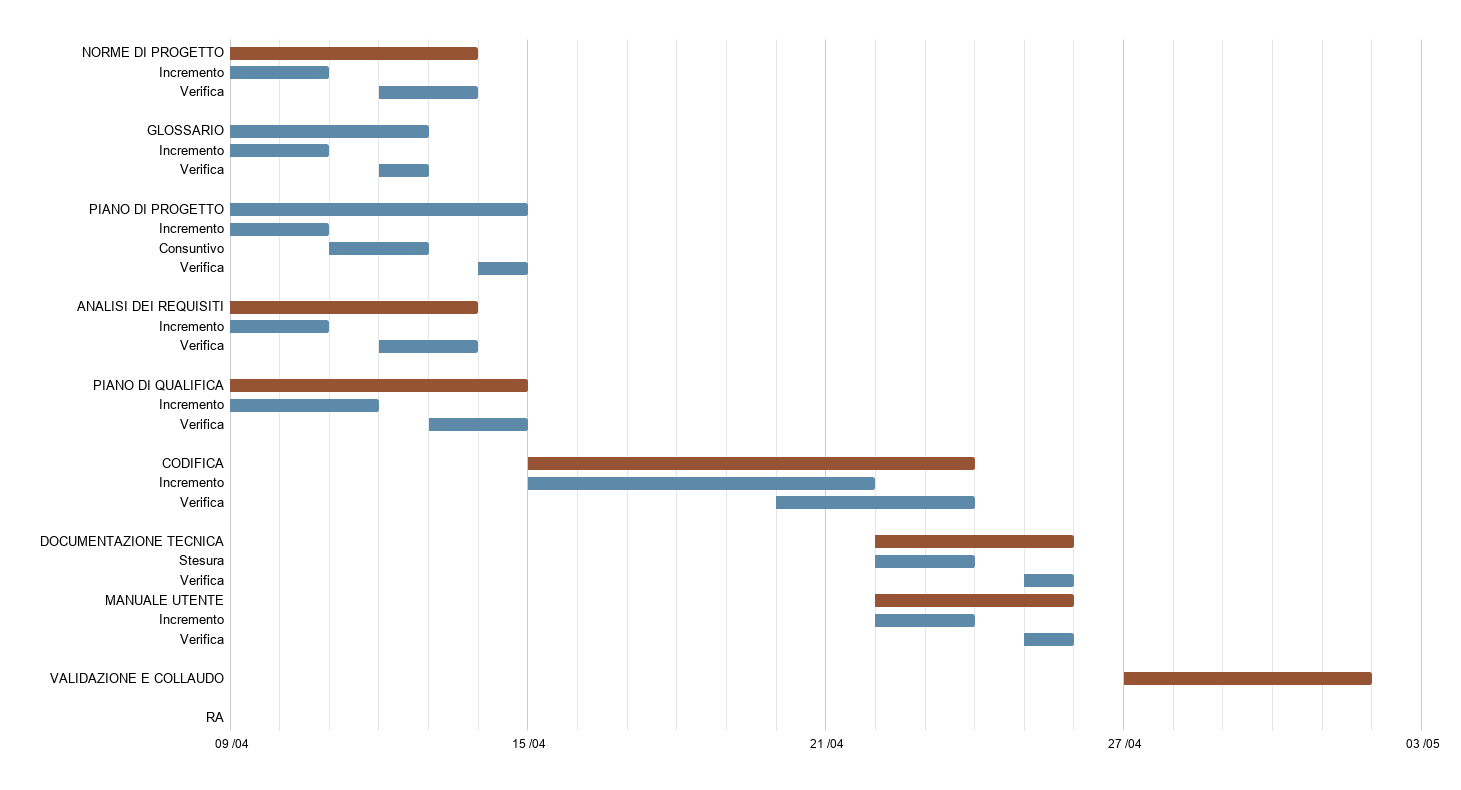
\includegraphics[width=0.8\linewidth]{../immagini/pdp/gantt_validazione.png}
		\caption{Diagramma di Gantt dell'attività di validazione e collaudo}
	\end{center}
\end{figure}
